\chapter{Measurements}

In this chapter we present the various measurements conducted with the
optical setup described in XX.

\section{Intensity Control}

The laser intensity is regulated by a control loop and \gls{aom} in order to
intercept power drifts from the laser source. In this section we want to
discuss the grade of this control loop and estimate an error in subsequent
intensity measures.

\subsection{Long term measurement}

As a start we measured the intensity with a second photodiode over the period
of over \SI{16}{\hour} in an interval of about \SI{2}{\minute}. The measured
intensity timeline is shown in \Cref{fig:intensity_control_long} and the
associated descriptive statistics in \Cref{tab:intensity_control_long}.

\begin{figure}[ht]
  \centering
  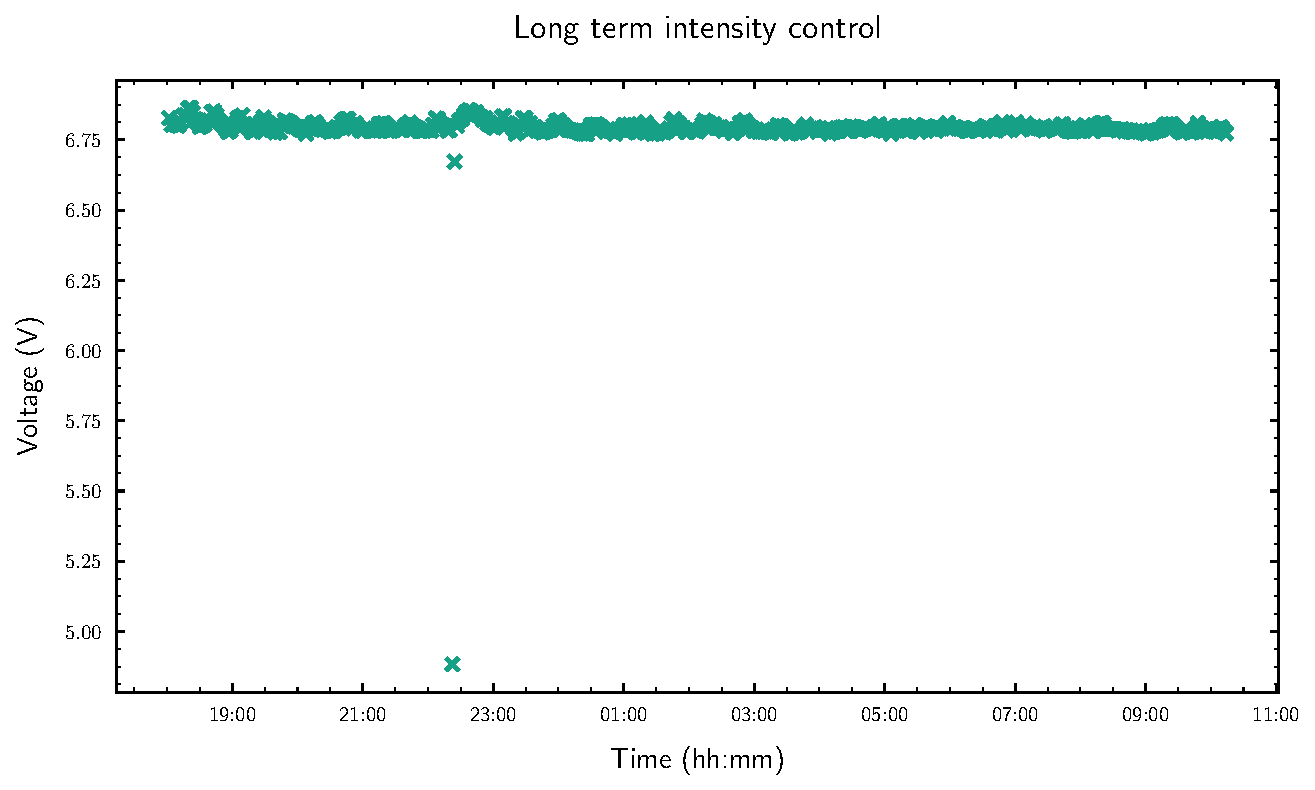
\includegraphics[width=.9\textwidth]{\figuredir{intensity/control-long.pdf}}
  \captionsetup{width=.7\textwidth}
  \caption{Long term measurement of the intensity with controlled intensity.
    The intensity was measured every \SI{2}{\minute} for over \SI{16}{\hour}
    to determine the accuracy of the intensity controller. The outlier at
    about 22:45 was caused by laboratory visit otherwise the intensity remains
  stable.}
  \label{fig:intensity_control_long}
\end{figure}

We can observe some outliers at about 22:45 which are probably caused by a
late laboratory visit, however we can not assure for a specific reason.

\begin{table}[h]
  \centering
  \begin{tabular}{|c|c|c|c|}
    \hline
    Mean & Minimum & Maximum & Standard deviation \\
    \hline
    \SI{6.79}{\volt} &
    \SI{4.88}{\volt} &
    \SI{6.86}{\volt} &
    \SI{0.09}{\volt} \\
    \hline
  \end{tabular}
  \captionsetup{width=.7\textwidth}
  \caption{Descriptive statistics of the short term measurement of the
  intensity with controlled intensity. Note the small standard deviation.}
  \label{tab:intensity_control_long}
\end{table}

\subsection{Short term measurement}

The previous section gave us already some good insights about the long term
stability of the intensity control loop. Yet in practice typical intensity
measurements are of much smaller magnitude, henceforth it seems close at hand
to measure short term effects too.

\begin{figure}[ht]
  \centering
  \captionsetup{width=.7\textwidth}
  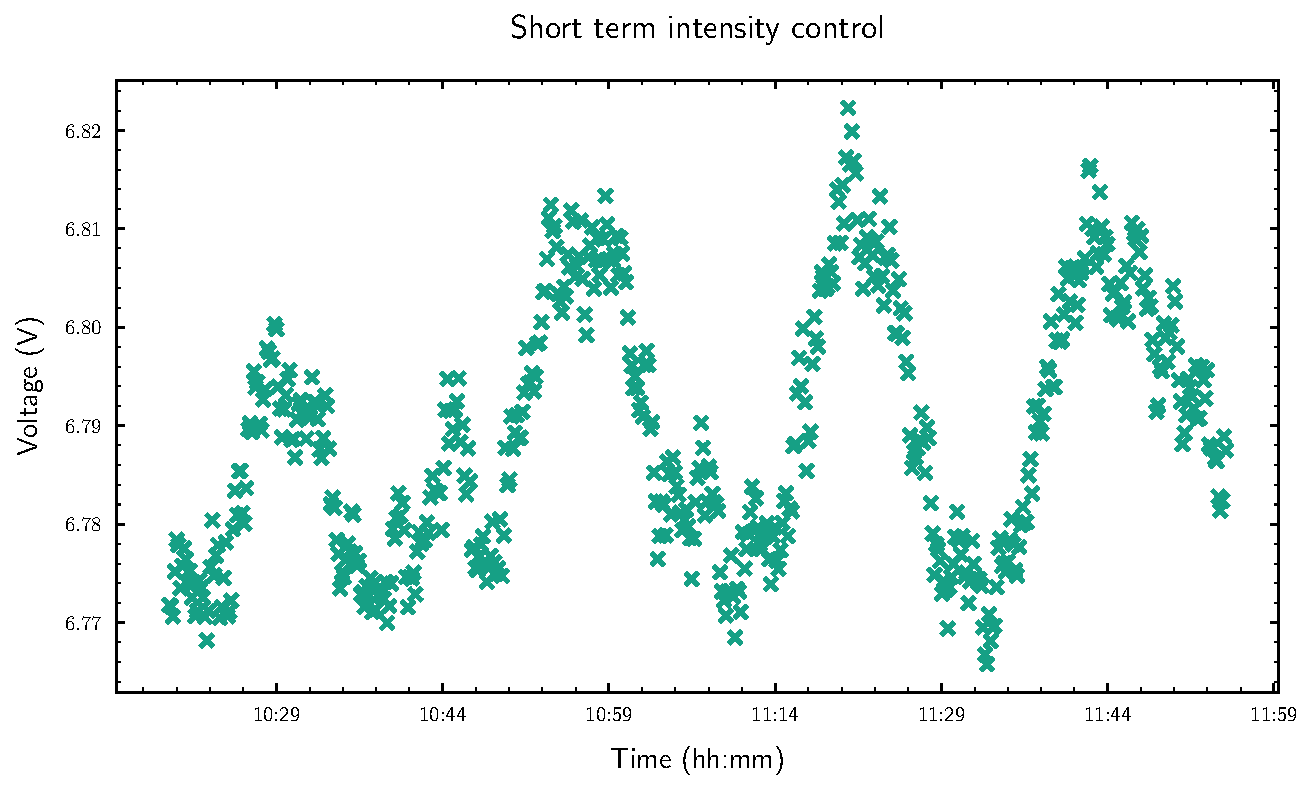
\includegraphics[width=.9\textwidth]{\figuredir{intensity/control-short.pdf}}
  \caption{Short term measurement of the intensity with controlled intensity.
    The intensity was measured every \SI{10}{\second} for over \SI{1}{\hour}
    to determine the accuracy of the intensity controller.}
  \label{fig:intensity_control_short}
\end{figure}

For short term measurements we used the same setup as for the long term
measurements. The time parameters now changed to a sample interval of
\SI{10}{\second}. The intensity timeline of the short term measurement is
depicted in \Cref{fig:intensity_control_short} and the associated descriptive
statistics are presented in \Cref{tab:intensity_control_short}.

On a smaller timescale we see that the intensity control loop performs
oscillations. The descriptive statistics show much smaller deviation from
the mean than observed in the long term measurements.

\begin{table}[h]
  \centering
  \begin{tabular}{|c|c|c|c|}
    \hline
    Mean & Minimum & Maximum & Standard deviation \\
    \hline
    \SI{6.78}{\volt} &
    \SI{6.77}{\volt} &
    \SI{6.82}{\volt} &
    \SI{0.01}{\volt} \\
    \hline
  \end{tabular}
  \captionsetup{width=.7\textwidth}
  \caption{Descriptive statistics of the short term measurement of the
  intensity with controlled intensity. Note the small standard deviation.}
  \label{tab:intensity_control_short}
\end{table}

\subsection{Comparison and error estimate}

Even though the previous analysis gave us a good picture of the magnitude
of intensity drifts on different time scale and confirms that the intensity
is in general regulated. Nevertheless we cannot make any statements with
regard to an error estimate without being able to compare the deviation
quantities to actual measurement data.

Because a typical measurement involves \gls{aod} that naturally cause an
intensity difference to the free path configuration we subtracted the
respective mean intensity so the following quantities only account for a
deviation from the respective mean. \Cref{tab:intensity_control} shows the
descriptive statistics of the long and short term measurements of the
intensity control with a typical intensity measurement. Comparing the
standard deviation of short term measurement with the standard deviation of a
typical intensity measurement yields us an approximate error of about
\SI{3}{\percent}. In \Cref{fig:intensity_control} we have the boxplots of
the absolute deviation from the respective mean intensity for the former
three measurement cases to visualize the spread and quantiles of the
intensity.

We conclude that the harmonic noise of the intensity control is in general
small enough to be neglected in further intensity discussion. Nevertheless
the usual intensity drifts may make it difficult to create high-precision
optical potentials.

\begin{table}[h]
  \centering
  \begin{tabular}{|c|c|c|}
    \hline
    Measurement & Value range & Standard deviation \\
    \hline
    long term & \SI{1.98}{\volt} & \SI{0.09}{\volt} \\
    \hline
    short term & \SI{0.06}{\volt} & \SI{0.01}{\volt} \\
    \hline
    typical & \SI{1.43}{\volt} & \SI{0.40}{\volt} \\
    \hline
  \end{tabular}
  \captionsetup{width=.7\textwidth}
  \caption{Descriptive statistics of the short and long term measurement
  of the intensity control and a typical intensity measurements where we
subtracted the mean intensity for comparison.}
  \label{tab:intensity_control}
\end{table}

\begin{figure}[ht]
  \centering
  \captionsetup{width=.7\textwidth}
  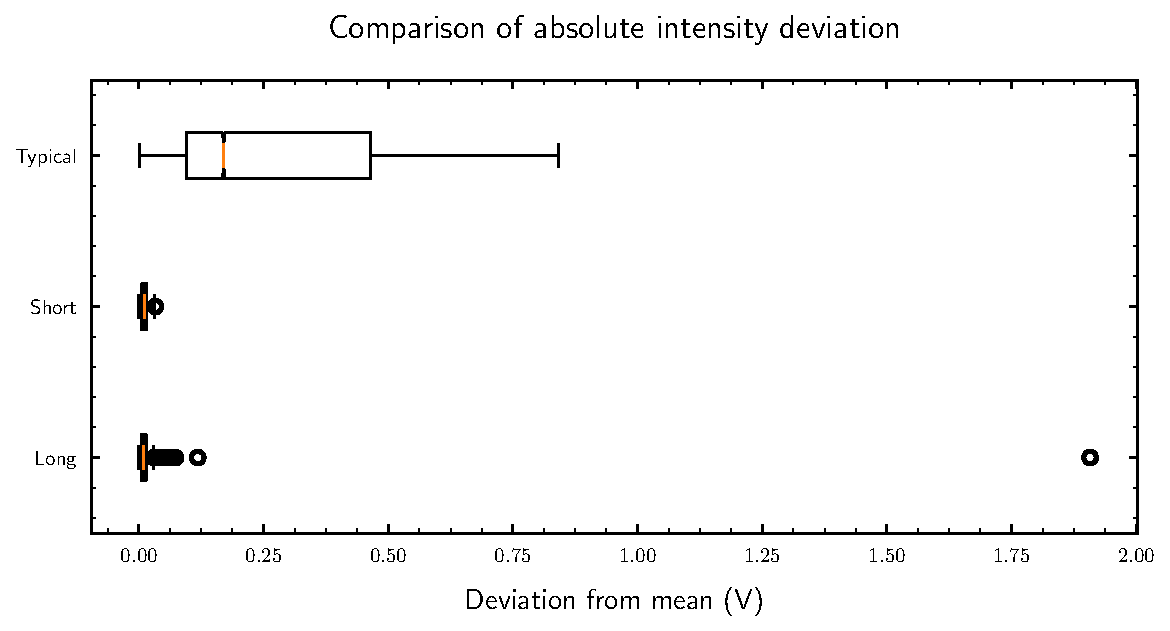
\includegraphics[width=.9\textwidth]{\figuredir{intensity/control-deviation.pdf}}
  \caption{Boxplot of the long and short term intensity measurements and a typical
  intensity measurement with the \gls{aod} where we subtracted the mean intensity
  for comparison. The typical measurements covers a much wider intensity range
then deviations from the intensity control loop.}
  \label{fig:intensity_control_comparison}
\end{figure}

\section{Synthesizer}

\begin{figure}[ht]
  \centering
  \captionsetup{width=.8\textwidth}
  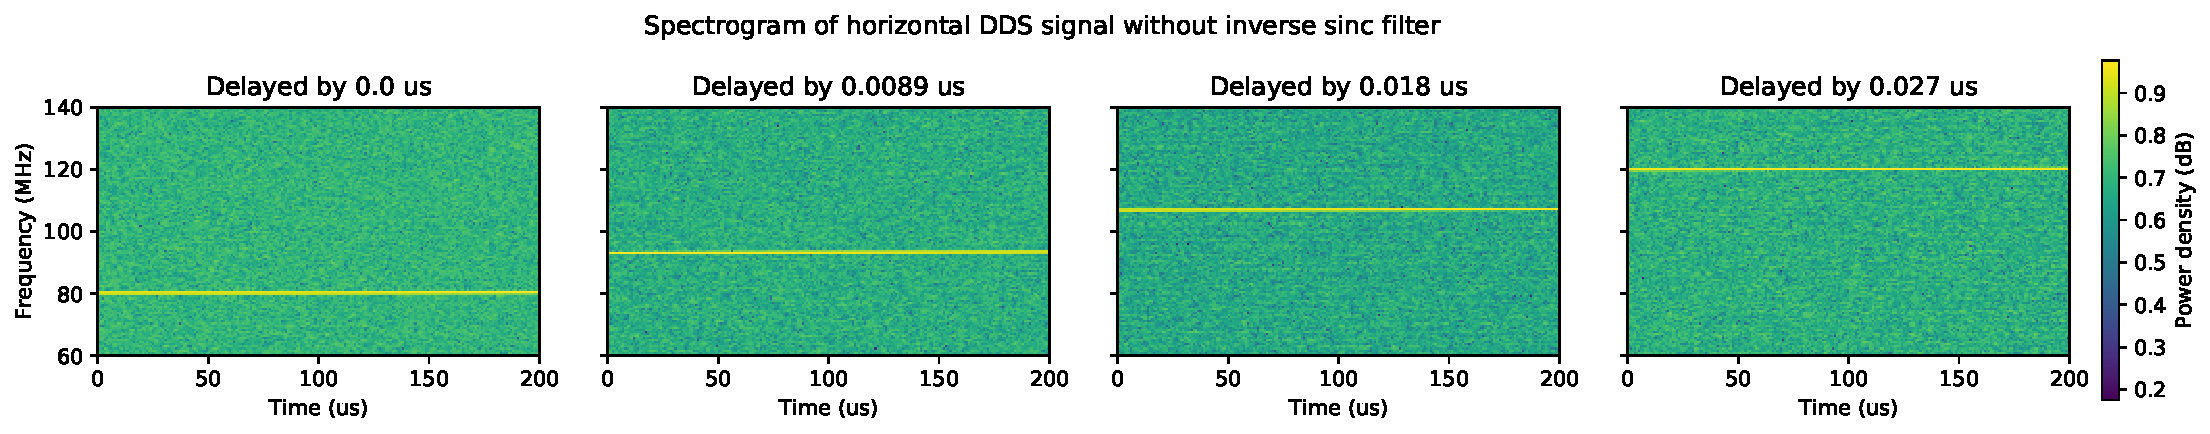
\includegraphics[width=\textwidth]{\figuredir{synthesizer/specgram.pdf}}
  \caption{Short measurement of the intensity without any electro-optics every
  \SI{10}{\second} for over \SI{1}{\hour} to determine the accuracy of the
  intensity controller.}
\end{figure}

\begin{figure}[ht]
  \centering
  \captionsetup{width=.8\textwidth}
  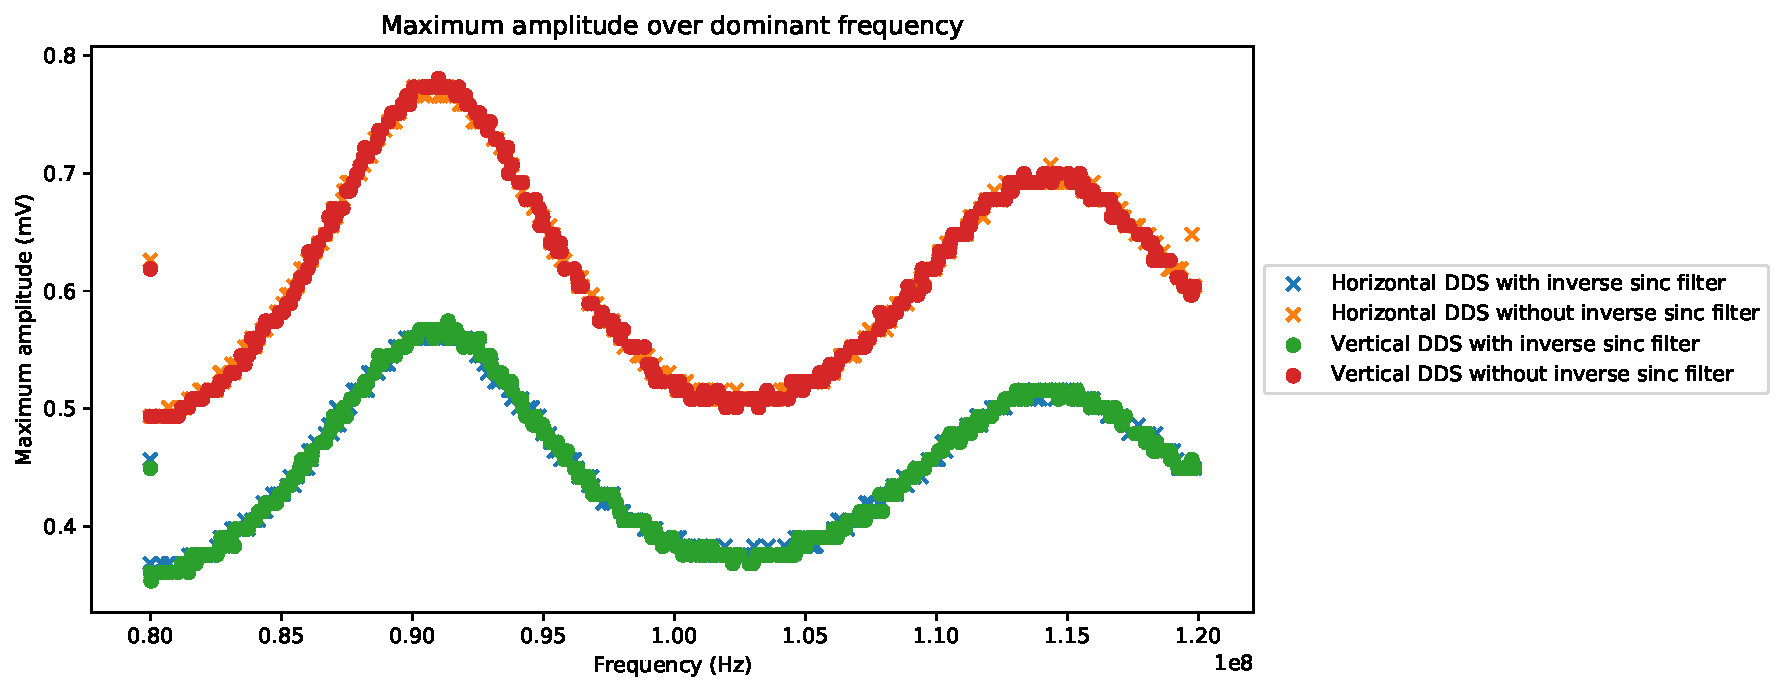
\includegraphics[width=\textwidth]{\figuredir{synthesizer/frequency.pdf}}
  \caption{Short measurement of the intensity without any electro-optics every
  \SI{10}{\second} for over \SI{1}{\hour} to determine the accuracy of the
  intensity controller.}
\end{figure}

\section{Amplifier}

\section{Acousto-optic deflector}
\subsection{Power matching}

\subsection{Intensity}
% H removed, V sweep (H in V position, vice versa)
% V removed, H sweep (V in H position, vice versa)

% H constant with V sweep
% V constant with H sweep

\chapter{Intensity Optimization}
\
% at different amplitude values
% without amplitude modulation
% with amplitude modulation
